% =============================================================================
%  Supplementary Section S1: Model.
%  Order of subsections: biology; the balance and the three hypotheses;
%  structural identifiability; the line geometry (Supplementary Fig. S1, which
%  must be the first figure of the SI); the carnitine model in detail; the
%  parameter registry. The carnitine-model subsection follows the line geometry
%  so that its figure is numbered after Supplementary Fig. S1.
% =============================================================================
\section{Model}
\label{si:s1}

This section sets out what the model represents and what it leaves out
(Section~\ref{si:s1-bio}), its equations under the three hypotheses for the non-enzymatic
route (Section~\ref{si:s1-eq}), when residual capacity is structurally identifiable
(Section~\ref{si:s1-si}), the geometry of a record of settled blood draws
(Section~\ref{si:s1-pencil}), the carnitine model in detail (Section~\ref{si:s1-carn}) and
a registry of every constant with what its value rests on
(Section~\ref{si:s1-reg}, Supplementary Table~\ref{stab:params}). Throughout, metabolite
levels are in \textmu M, capacities, loads and delivered increments are fluxes in \um, rate
constants are in d$^{-1}$ and times are in days.

% -----------------------------------------------------------------------------
\subsection{What the model represents}
\label{si:s1-bio}

\paragraph{Where propionyl-CoA comes from.} Propionyl-CoA is formed in the mitochondria from
the catabolism of isoleucine, valine, methionine and threonine, from odd-chain fatty acids
and from propionate made by gut bacteria. In patients with disorders of propionate metabolism, amino-acid catabolism supplied a mean of 51.7\% of propionate
production (range 24.5--66.4\%), gut bacteria at least 22.2 $\pm$ 8.5\% (estimated from
the fall under metronidazole), and about 30\% was unaccounted for and attributed to
odd-chain fatty acids~\cite{propionate_sources}. Protein restriction lowers the first
share and intestinal antibiotics the second. Decompensations are usually triggered by an
intercurrent illness~\cite{pa_guidelines}, during which the breakdown of muscle protein
raises the amino-acid share even when the patient is not eating.
% src: paper/sections/01_biology.tex:149-156 (catabolism during illness); src/common/params.py:496-505 (s_base row: 51.7%, 24.5-66.4%, 22.2 +/- 8.5%, ~30%)

\paragraph{The enzyme route.} Propionyl-CoA carboxylase (PCC) is a biotin-dependent
mitochondrial enzyme built from $\alpha$ and $\beta$ subunits, encoded by \emph{PCCA} and
\emph{PCCB}~\cite{pcc_structure}. It carboxylates propionyl-CoA to methylmalonyl-CoA,
which is converted further to succinyl-CoA and enters the tricarboxylic acid
cycle~\cite{pa_guidelines}. In propionic acidaemia (PA) the residual
activity measured in patients' cultured fibroblasts is typically a few per cent of
control~\cite{pcc_residual_activity}. The mRNA therapy makes hepatocytes produce
functional PCC~\cite{jiang2020dual,mrna_moa}, so after each infusion the liver's enzyme
capacity is the patient's own plus a delivered increment that decays as the protein is
turned over.
% src: paper/sections/01_biology.tex:7-13 (alpha6beta6, PCCA/PCCB, C01; claims.csv C01); claims.csv C52 (under 5% of control, fibroblasts); manuscript/main.tex:94-99 (residual activity; mRNA-3927), :576-578 (methylmalonyl-CoA to succinyl-CoA, pa_guidelines)

\paragraph{The carnitine route.} When PCC is deficient, propionyl groups are transferred to
carnitine to form propionylcarnitine, which leaves the cells and is excreted in urine. Each
propionyl group removed in this way takes one carnitine molecule with it, so the route
consumes its own carrier. In two patients with PA and two with methylmalonic aciduria,
urinary free carnitine was decreased while urinary short-chain acylcarnitines, mostly
propionylcarnitine, were increased~\cite{carnitine_excretion_pa}, and in a child with PA
plasma free carnitine was 5.7\uM\ against a normal $37\pm8$\uM~\cite{carnitine_pa_child}.
This secondary carnitine deficiency is why carnitine is supplemented.
% src: paper/claims.csv:37 (C41, Di Donato: two PA, two MMA); paper/claims.csv:24 (C25: 5.7 uM vs 37 +/- 8); paper/sections/03_dynamic.tex:29-35

\paragraph{Renal recovery of carnitine, and competition from acylcarnitines.} Filtered free
carnitine is normally recovered from the glomerular filtrate by a transporter in the renal
brush-border membrane. In a carnitine transporter solubilised from rat renal brush-border
membranes and reconstituted into liposomes, acylcarnitines were the most effective
inhibitors of carnitine transport, and besides carnitine only acylcarnitines and betaine
were efficiently translocated~\cite{octn2_renal_transport}. If the same competition
operates in patients, a rise in propionylcarnitine lowers the fraction of filtered carnitine
that is recovered, so the free carnitine pool acquires a second exit that widens as the
metabolite accumulates. This step of the model rests on one in vitro study in the rat; no
measurement in patients shows the recovered fraction falling as propionylcarnitine rises.
% src: paper/claims.csv:38 (C42: rat, in vitro, reconstituted; no patient measurement); paper/sections/03_dynamic.tex:44-53

\paragraph{What the single metabolite stands for.} Accumulated propionyl-CoA also gives rise
to 3-hydroxypropionate (3-HP), 2-methylcitrate (2-MC) and propionylglycine, which appear in
blood and urine; the measured urinary output of propionate metabolites in PA is a few per
cent of estimated production~\cite{thompson1990fasting}. The model carries one metabolite,
$m$, identified with plasma 3-HP. It stands for the pool of accumulated propionyl
metabolites and is assumed to rise and fall monotonically with intracellular propionyl-CoA,
the enzyme's true substrate, which is not measured. 3-HP is used because it is associated
with outcome, a 50\% lower concentration carrying a decompensation rate ratio of 0.7 (95\%
CI 0.6--0.9) where 2-MC carried none~\cite{natural_history}, and because it is not a
carnitine conjugate, so carnitine supplementation does not raise it directly as it raises
propionylcarnitine. Because $m$ is a plasma marker, the half-saturation $K_m$ of
the enzyme term is a shape constant of clearance at the plasma level, not the in vitro
Michaelis constant of PCC for propionyl-CoA (0.29\,mM~\cite{pcc_liver_kinetics}).
% src: paper/sections/02_model.tex:334-345 (marker remark, rate ratio 0.7, CI 0.6-0.9, 2-MC 1.0); paper/claims.csv C19 (C3 also carries RR 0.6, so 3-HP is not the only marker with an outcome association), C49; paper/sections/01_biology.tex:111-118; src/common/params.py:176-180 (K_m row, 0.29 mM); manuscript/main.tex:584-586

\paragraph{What is not represented.} The model has no propionyl-CoA state and no
intracellular compartment, so propionylcarnitine, 2-MC and propionylglycine are not
represented as separate species. Coenzyme A has no state either: the linear- and
saturable-clearance models carry nothing for its sequestration by accumulated
propionyl-CoA, and the carnitine model carries a feedback of the same kind only through
carnitine, the carrier that conjugation consumes. The inhibition of the urea cycle that
leads to hyperammonaemia~\cite{pathophys_complications} is not represented, so the model
describes the accumulation of the metabolite and the capacity that clears it, and leaves
out the ammonia arm of a crisis. Bicarbonate, the second substrate of PCC, is held constant. The kinetics of mRNA
translation are replaced by a jump in enzyme capacity at each infusion that then decays
exponentially, and the immune response to the lipid nanoparticle carrier is outside the
model. In the carnitine model, the carnitine state is the carnitine available for
conjugation, not plasma free carnitine. Supplementary Table~\ref{stab:s1-biomap} summarises
the correspondence.
% src: paper/sections/01_biology.tex:109-145 (reduction's cost: substrate not modelled, urea cycle; CoA sequestration absent from the reduced structures, the dynamic model reintroduces the cofactor-consuming feedback through carnitine); paper/claims.csv C02, C03 (pathophys_complications: matches-with-drift, cited for the complications, not for the NAGS step); paper/sections/A1_supplementary.tex:28 (bicarbonate held constant); manuscript/main.tex:587-589

\begin{table}[tbp]
\centering
\footnotesize
\renewcommand{\arraystretch}{1.15}
\caption{\label{stab:s1-biomap}What each element of the model stands for. ``All'' means the
element is shared by the linear-clearance, saturable-clearance and carnitine models.}
\begin{tabular}{@{}>{\raggedright\arraybackslash}p{0.31\linewidth}>{\raggedright\arraybackslash}p{0.19\linewidth}>{\raggedright\arraybackslash}p{0.11\linewidth}>{\raggedright\arraybackslash}p{0.31\linewidth}@{}}
\toprule
biology & model element & model & status \\
\midrule
propionate from protein, odd-chain fatty acids and gut bacteria & load $L(t)+L_0$ & all &
$L(t)$ from the diet record; $L_0$, the unrecorded part, an unknown constant \\
the patient's own PCC & $\theta\,g(m)$ & all & $\theta$ is the estimand; Michaelis--Menten
form \\
PCC made from the infused mRNA & $\Delta(t)\,g(m)$ & all & a known input on the enzyme exit;
its size $D$ and decay rate $\lambda$ are assumed \\
plasma 3-HP & $m$ & all & the observation; a proxy for propionyl-CoA \\
conjugation to carnitine and urinary loss of propionylcarnitine & $\alpha(m)$ & all &
three hypotheses for its shape \\
available carnitine and its replenishment (diet, synthesis, supplements) & $c$, $R_0$ &
carnitine & not observed; $R_0$ derived from a calibration \\
urinary loss of free carnitine, widened by acylcarnitine competition & $\delta(m)\,c$ &
carnitine & competition shown in vitro, rat~\cite{octn2_renal_transport} \\
propionyl-CoA, coenzyme A, ammonia & none & none & not represented; cofactor depletion
enters the carnitine model only through carnitine \\
\bottomrule
\end{tabular}
\end{table}

% -----------------------------------------------------------------------------
\subsection{The balance and the three hypotheses for the non-enzymatic route}
\label{si:s1-eq}

\paragraph{The shared balance.} The metabolite level $m(t)$ obeys
\begin{equation}
\label{seq:s1-balance}
\dot m \;=\; L(t) + L_0 \;-\; \bigl(\theta+\Delta(t)\bigr)\,g(m) \;-\; \alpha(m),
\qquad g(m)=\frac{m}{K_m+m}.
\end{equation}
$L(t)$ is the recorded propiogenic load, the part of the inflow that the diet record
documents. $L_0$ is the unrecorded part, carried as an unknown constant; it enters every fit
as an offset $b$ on the recorded load. $\theta$ is the residual capacity, the maximal flux
the patient's own PCC can carry, on a scale on which normal capacity is 3000\um. $g(m)$ is
the fractional saturation of the enzyme, with half-saturation $K_m$, and $\alpha(m)$ is the
non-enzymatic route. $\theta$ absorbs the maximal velocity: writing the enzyme term as
$V_{\max}\,\theta\,g(m)$ would add a parameter that no record of $m$ can separate, because
only the product multiplies $g$.
% src: manuscript/main.tex:593-604; paper/sections/02_model.tex:59-66 (theta absorbs V_max)

\paragraph{The delivered increment.} Each infusion adds to the enzyme's maximal flux,
\begin{equation}
\label{seq:s1-delta}
\Delta(t) \;=\; D\sum_{k:\,t_k\le t} e^{-\lambda(t-t_k)},\qquad \lambda=\frac{\ln 2}{t_{1/2}},
\end{equation}
over past infusions at times $t_k$. $D$ is the jump at each fortnightly infusion, assumed to
be 6000\um\ (twice normal capacity; the ``assumed dose''), and $t_{1/2}$ is the half-life of
the delivered PCC protein: 3.5\,d, an assumed design value, in the identifiability and
sampling analyses, and about 4.3\,d as the likely hepatic value (Supplementary
Section~\ref{si:s6:halflife}). For comparison, the intrinsic PCC decay of the translational
model corresponds to 3.8\,d and its stated protein half-life is about
7\,d~\cite{pkpd_translational}. On a fortnightly
schedule ($T=14$\,d) the increment settles to a periodic pattern with peak
$D/(1-e^{-\lambda T})$ just after each infusion and trough
$D\,e^{-\lambda T}/(1-e^{-\lambda T})$ just before the next: 6400 and 400\um\ at a 3.5-day
half-life, against a normal capacity of 3000\um. Because the increment multiplies the same
saturation $g(m)$ as the patient's own enzyme, the infusions act on the enzyme exit alone,
and their known, repeated rise and decay is what makes the routine record an
identification experiment.
% src: manuscript/main.tex:599-604, :654 (3.5 d assumed; intrinsic decay 3.8 d); audit/brief_2026-10-01/REPORT.md:1004 (Attarwala k_deg 0.0075/h, 3.8 d intrinsic, effective terminal ~7 d); src/common/params.py:283-300 (stated protein half-life ~7 d); out/t44_interval_decision.txt:4-5 (Delta_trough(14)=400.0, Delta_peak(14)=6400.0)

\paragraph{The ceiling.} We require that the patient's own capacity plus the delivered
enzyme never exceed normal, as a plausibility condition of the model rather than a measured
toxicity limit. Set for a patient at 5\% of normal (150\um), it caps the delivered peak at
2850\um. The largest dose within the ceiling, and how far the assumed dose exceeds it, are
derived in Supplementary Section~\ref{si:s6:ceiling}.
% src: manuscript/main.tex:753-755 (2850); the capped dose 2672 and the 2.18 times normal are in s6_interval.tex (si:s6:ceiling), sourced there to out/t53_crossing_shape.txt:65,87 and out/t44_interval_decision.txt:5

\paragraph{Three hypotheses for the non-enzymatic route.} How the non-enzymatic route
behaves in PA is not established, so $\alpha$ is given three forms:
\begin{equation}
\label{seq:s1-alphas}
\begin{gathered}
\alpha_{\mathrm{lin}}(m)=k_e\,m,\qquad
\alpha_{\mathrm{sat}}(m)=\frac{V_e\,m}{K_e+m},\\[4pt]
\alpha_{\mathrm{carn}}(m)=\frac{R_0\,u(m)}{u(m)+\rho(m)},\qquad
u(m)=\frac{m}{K_c+m},\qquad \rho(m)=\rho_0\Bigl(1+\frac{m}{M_i}\Bigr).
\end{gathered}
\end{equation}
With constant inputs, a steady state is a level at which the total clearance
$C(m)=(\theta+\Delta)\,g(m)+\alpha(m)$ equals the inflow $L+L_0$; it is stable where $C$ is
increasing. Each hypothesis is used for a stated purpose rather than as one step in a sequence
of approximations: the linear-clearance model for identifiability and sampling design, the
saturable-clearance model to test which conclusions depend on a straight line, and the
carnitine model for the dosing interval and late infusions.
% src: manuscript/main.tex:186-206,604-610

\paragraph{The linear-clearance model.} Here $\alpha=k_e m$ with $k_e=5$\,d$^{-1}$; on its
own the route would clear the marker with a half-life of $\ln2/k_e=3.3$\,h. The operating
point is a marker level $\bar m=10$\uM\ at normal capacity, which fixes the load at
$L=\theta g(\bar m)+k_e\bar m=272.7+50=322.7$\um. The load is held there as capacity falls,
so that at 5\% of normal the untreated steady state is $m=54.0$\uM\ and the enzyme carries a
share $s=\theta g(m)/L=0.163$ of the load, the route the other 84\%; at normal capacity the
enzyme's share is 84.5\%. Because the route is unbounded, a steady state exists at every
$\theta\ge0$ and there is no tipping point. A threshold must therefore be defined by
convention, as the capacity at which an illness load $fL$ holds the marker exactly at a
tolerable level $m_{\mathrm{tol}}$,
\begin{equation}
\label{seq:s1-thcritlin}
\theta_{\mathrm{crit}}^{\mathrm{lin}}=\frac{fL-k_e\,m_{\mathrm{tol}}}{g(m_{\mathrm{tol}})},
\end{equation}
which is 430\um\ at $f=1$ and 994\um\ at the illness fold $f=1.5$, with
$m_{\mathrm{tol}}=40$\uM. The linear-clearance model is not a linearisation of the carnitine
model. At the carnitine model's operating point the tangent to its clearance has an
intercept to which the non-enzymatic route contributes 374\um, against 61\um\ from the
enzyme, and
fitting $k_e m$ to the carnitine model's own clearance from its operating point to eight
times it puts $\hat k_e$ on its lower bound of zero ($-0.36$ if released). A straight route
is kept because it is the shape most easily told apart from the enzyme's curve, which makes
it the favourable case for identification.
% src: src/common/params.py:47-57 (k_e=5/d is a 3.3 h half-life), :101 (M_OP 10, M_TOL 40, ILLNESS_FOLD 1.5); src/common/models.py:68-74; audit/brief_2026-10-01/REPORT.md:147 (L = 322.73, m = 54.0, s = 0.163 at 5%); results/numbers/scope.tex:25 (share_5pct 16.3) and share_nominal_pct 84.5; out/t44_interval_decision.txt:40,64 (theta_crit 994.3 at fold 1.5, 430 at fold 1.0); paper/sections/03_dynamic.tex:304-315 (374 vs 61); paper/sections/02_model.tex:259-263 (fit_band_top 8, fit_ke_hat_free -0.36)

\paragraph{The saturable-clearance model.} Here $\alpha=V_e m/(K_e+m)$, with $V_e$ the
route's maximal rate (a flux, not the linear $k_e$) and $K_e$ its half-saturation. Total
clearance now levels off towards $\theta+V_e$, so a steady state exists only while
$L+L_0<\theta+V_e$, and it is lost by escaping to ever higher levels rather than by the
collision of two steady states. At the model's nominal constants, $V_e=400$\um\ and
$K_e=300$\uM, the load that places the marker at 10\uM\ at normal capacity is 285.6\um,
below $V_e$, so a patient with no enzyme of their own could be maintained, which is not the
severe phenotype. We therefore also use a constructed operating point with $V_e=100$\um,
below the untreated load of about 276\um, and a managed load of 220\um, about 20\% lower. A
patient at 5\% of normal then has a steady state, with a critical capacity
$L-V_e=120$\um\ (4.0\% of normal) and a margin of about 1\% of normal. Neither $V_e$ nor
$K_e$ has a source. At 5\% of normal the enzyme carries 0.37 of the load at the nominal
constants, against 0.16 in the linear-clearance model.
% src: src/common/models.py:78-83 (ParamsB ke=400 as V_max, Ke=300); audit/brief_2026-10-01/REPORT.md:752-758 (anchored load 285.6, 276.0; theta_crit = L - k_e), :764-772 (managed L 220: theta_crit 4.0%, margin +1.0%), :774 (B unregistered), :780-784 (share 0.16 vs 0.37); out/t35_managed_load.txt:48

\paragraph{The carnitine model.} $\alpha_{\mathrm{carn}}$ is the steady-state form of a
two-state system in which available carnitine is a second state. That system, its
reduction, the derivation of $R_0$ and the tipping point are in
Section~\ref{si:s1-carn}.

% -----------------------------------------------------------------------------
\subsection{Structural identifiability}
\label{si:s1-si}

Structural identifiability asks whether, with perfect noise-free data, only one parameter
vector reproduces the measurements. The answer for the linear-clearance model depends on
what the record contains: a followed trajectory, a single steady state, or many settled
draws under the infusions.

\paragraph{A followed trajectory.} Suppose $m(t)$ is measured exactly over an interval
during which it moves. Then $\dot m$ is known, and without therapy and with the load known
the function
\begin{equation}
\label{seq:s1-F}
F(m)\;=\;L-\dot m\;=\;\theta g(m)+k_e m\;=\;\frac{k_e m^2+(\theta+k_eK_m)\,m}{m+K_m}
\end{equation}
is known at every level visited. A rational function known on an interval fixes its
coefficients, here $(K_m,\;k_e,\;\theta+k_eK_m)$, and that triple determines
$(\theta,K_m,k_e)$ uniquely, so the model is globally structurally identifiable. Locally the
trajectory must visit at least three distinct levels, one per parameter. With therapy and an
unknown $L_0$ the same holds: only the therapy carries a term in $\Delta$, so $K_m$ follows
from that coefficient alone, and the remaining three parameters follow at three distinct
levels. Symbolic checks with \texttt{StructuralIdentifiability.jl} returned global
identifiability for every configuration tested (a generic input; a constant input started
away from steady state; two patients sharing $K_m$ and $k_e$; a carnitine dose acting on the
non-enzymatic route; the therapy acting on the enzyme; and the carnitine two-state model,
with carnitine never observed), with one exception, the saturable-clearance model, which is
only locally identifiable (below).
% src: paper/note_structural_identifiability.tex:96-145 (eq F, prop:global, rank condition), :417-441 (cases A1-A6, B, C); paper/sections/06_excitation.tex:11-17

Identifiable in principle is not the same as precise. At $(\theta,K_m,k_e)=(3000,100,5)$ the
condition number of the column-normalised sensitivity matrix falls roughly as the inverse
square of the relative excursion of the marker, from $2.7\times10^{6}$ at a 2\% excursion
to $1.1\times10^{5}$ at 10\% and $1.5\times10^{3}$ at 100\%. A well-managed patient, whose
marker moves by a few per cent between visits, presents a badly conditioned problem.
% src: paper/note_structural_identifiability.tex:166-198 (tab:cond and corollary)

\paragraph{A single steady state.} A patient seen only at one steady state supplies one
algebraic equation, $L=\theta g(m)+k_e m$, in three unknowns, so two directions remain
undetermined. Pooling patients does not close them: $N$ patients each seen at one steady
state and sharing $K_m$ and $k_e$ supply $N$ equations in $N+2$ unknowns, whatever $N$. The
symbolic result for a constant input does not contradict this, because there the marker
starts away from its steady state and relaxes over about four hours, a transient that a
clinic does not sample.
% src: paper/note_structural_identifiability.tex:208-228 (deficiency exactly 2, regardless of N), :449-459 (constant input vs constant state; about four hours)

\paragraph{Settled draws under the infusions: the routine record.} The marker settles about a
hundred times faster than the delivered enzyme decays (Supplementary
Section~\ref{si:s2:firsthour}), so every draw outside the first hour after an infusion sees the
marker at the steady state set by that day's load and increment.
Each draw $i$ is then a point on the algebraic balance
$(\theta+\Delta_i)\,g(m_i)+k_e m_i=L_i+b$, where $b$ is the offset that carries the
unrecorded load. Solving it for the increment that produces a level $m$ gives, with no
remainder,
\begin{equation}
\label{seq:s1-invariants}
\Delta(m)=\frac{A}{m}+B+C\,m,\qquad A=K_m(L+b),\quad B=L+b-\theta-k_eK_m,\quad C=-k_e .
\end{equation}
Because the infusions move $\Delta$ over a wide range, the draws visit many levels, and
three distinct levels determine $(A,B,C)$. At a constant recorded load, however, there are
four unknowns $(\theta,K_m,k_e,b)$ against three invariants, which leaves an exact
one-parameter family of parameter vectors that reproduce every draw:
\begin{equation}
\label{seq:s1-fibre}
K_m(b)=\frac{K_m^{0}L}{L+b},\qquad
\theta(b)=\theta^{0}+b+k_e\bigl(K_m^{0}-K_m(b)\bigr),\qquad k_e\ \text{unchanged},
\end{equation}
where the superscript 0 marks the true values. Read as a bias, a record generated at load
$L+b$ and fitted with the load held at $L$ returns
$\hat\theta=\theta-b\,(1+K_mk_e/L)$ exactly, $\theta-2.549\,b$ at the normal operating
point.
% src: paper/sections/06_excitation.tex:19-25 (timescale_ratio 104), :27-58 (eq:invariants, eq:fibrecl, bias map); results/numbers/design.tex:111 (timescale_ratio 104); results/numbers/fibre.tex:3 (bias_slope 2.549)

The same fact appears in the sensitivity columns. At a constant recorded load, the
derivatives of the balance with respect to $(\theta,K_m,k_e,b)$ satisfy one linear
dependence,
\begin{equation}
\label{seq:s1-nullvec}
n=\bigl(L+b+k_eK_m,\;-K_m,\;0,\;L+b\bigr),
\end{equation}
identically in $m$ and in $\Delta$. We call this the load-bias identity. The design matrix
is rank deficient by exactly one, the deficient direction runs through the load offset,
$k_e$ does not enter it, and because it holds for every $\Delta$ the dose train alone does
not remove it. A recorded load that varies from draw to draw ($L\to L_i$) does: $A$ and $B$
then change with the known $L_i$, and no sample-independent dependence remains. The
identity was confirmed numerically by two routes sharing no code (residual
$\lVert Qn\rVert/\lVert Q\rVert=2.7\times10^{-17}$ on the two-year record, $Q$ the design
matrix). In practice, at the 10\% day-to-day variation in intake assumed throughout, the
data fill the deficient direction and the prior on $b$ is nearly inert; at a few per cent
or less the prior carries it. What this requires of the intake record is set out in
Supplementary Section~\ref{si:s2:record}.
% src: paper/sections/06_excitation.tex:236-271 (prop:rank, eq:nullvec, 2.7e-17, two routes), :296-315 (variability fills the direction; prior on b inert at 10%); the advice not to smooth (06_excitation.tex:331-336) is given in s2_sampling.tex (si:s2:record); paper/sections/A1_supplementary.tex:166-210 (derivation)

\paragraph{The exchange symmetry of the saturable-clearance model.} When both exits have the
same Michaelis--Menten shape, $f(m;K)=m/(K+m)$, the total clearance is
$(\theta+\Delta(t))\,f(m;K_m)+V_e\,f(m;K_e)$. Without therapy,
\texttt{StructuralIdentifiability.jl} returns this model as locally but not globally
identifiable, with identifiable functions $\theta+V_e$, $K_m+K_e$, $\theta V_e$, $K_mK_e$
and $K_e\theta+K_mV_e$, every one unchanged by exchanging $(\theta,K_m)$ with $(V_e,K_e)$.
The true parameters and their channel-swapped image reproduce any record exactly. With the
increment kept on the enzyme exit, the swapped parameters change the clearance by
\begin{equation}
\label{seq:s1-swap}
C_{\mathrm{swap}}-C=\Delta(t)\,\bigl[f(m;K_e)-f(m;K_m)\bigr].
\end{equation}
A constant increment $\Delta=c$ does not break the symmetry, because it is absorbed into
the amplitudes ($\theta'=V_e-c$, $V_e'=\theta+c$ reproduce the record exactly); the symbolic
tool again returns only local identifiability. An increment that varies in time does break
it whenever $K_e\ne K_m$, because $f(\cdot;K_e)$ and $f(\cdot;K_m)$ are then linearly
independent, and the tool returns global identifiability. The fortnightly rise and decay of
$\Delta(t)$ is such an input. Two qualifications follow. First, with three or more exits of
the same shape, one varying input breaks only the exchanges that involve the exit it drives.
Second, the linear-clearance model escapes the symmetry for a different reason, namely that
its two exits are not members of one family, so there is no exchange to break. Removing the symmetry
does not make the saturable-clearance model precise; its practical identifiability is in
Supplementary Section~\ref{si:s4:sat}.
% src: paper/sections/A1_supplementary.tex:560-600 (eq:modelB, eq:Binvariants), :605-660 (prop:exchange, constant-increment repair a1'=a2-c, n>=3 case); paper/note_structural_identifiability.tex:435-438,466-475

% -----------------------------------------------------------------------------
\subsection{The line geometry of settled draws}
\label{si:s1-pencil}

Moving the known increment to the right-hand side of the balance turns each settled draw
into a straight line in the plane of residual capacity and the non-enzymatic rate constant,
\begin{equation}
\label{seq:s1-pencil}
g(m_i)\,\theta+m_i\,k_e=L(t_i)+L_0-\Delta_i\,g(m_i),
\qquad \frac{dk_e}{d\theta}=-\frac{g(m_i)}{m_i}=-\frac{1}{K_m+m_i}.
\end{equation}
Every point on line $i$ explains draw $i$ exactly. Without noise, at the true $K_m$ and with
$L_0$ known, all the lines pass through the true $(\theta,k_e)$ (checked to
$2.5\times10^{-12}$). With assay and load-record error they nearly meet, and the region in
which they nearly meet is the uncertainty of $(\theta,k_e)$ at fixed $K_m$. The slope of
each line depends only on that draw's marker level, so draws at similar levels give nearly
parallel lines, which cross along a long sliver rather than at a point.
% src: audit/brief_2026-10-01/REPORT.md:1086-1090 (line form, concurrence); out/t51_pencil_geometry.txt:10-11

Supplementary Fig.~\ref{sfig:pencil}a shows the monthly record at 5\% of normal ($\theta=150$\um,
$k_e=5$\,d$^{-1}$, $K_m=100$\uM): 25 monthly draws over two years on therapy, with observed
marker levels of 4.3--37.8\uM. Every slope lies between about $-0.0096$ and $-0.0074$, so
the lines run almost parallel. Weighted by their noise, the region where they nearly meet
has a correlation between $\ln\theta$ and $\ln k_e$ of $-0.998$, an aspect ratio of 29 to 1,
and a standard deviation of $\ln\hat\theta$ of 2.73, with $K_m$ and $L_0$ known and no prior
on $k_e$. This near-parallelism is the correlation of $-0.99$ reported in the main text. On
the noiseless profile likelihood at 5\% of normal, a capacity close to zero or twice the
truth is matched by moving $k_e$ only about 20\% either way (to 6.11 and 3.89\,d$^{-1}$
from 5). Letting $K_m$ vary as well slides the meeting point along a curve. Adding that
freedom and the unknown load offset, together with the prior on $k_e$, gives the main text's
standard deviation of 3.05--3.07 (the two values differ only in the noise model;
Supplementary Section~\ref{si:s8-how}).
% src: out/t51_pencil_geometry.txt:6 (m_obs 4.3-37.8), :10 (slopes, true levels), :17 (-0.998, 29.0, 2.73); out/t1_identifiability.txt:25 (corr -0.9919, 3.0673), :59,:62 (k_e on the profile 6.108 at 0.01x, 3.885 at 2x); REPORT.md:1097, 1111 (fibre adds to the fixed-K_m ellipse)

Supplementary Fig.~\ref{sfig:pencil}b shows an imagined record that could not be run. The 25
draws are taken instead at 25 untreated steady states, under daily loads set evenly from 0.45
to 3.2 times the usual recorded load (145--1033\um\ against 323\um). The marker then ranges
over 23.8--188.9\uM, the slopes fan out, and the lines meet at a visible angle: the
correlation is $-0.969$, the aspect ratio 8 to 1, and the standard deviation of
$\ln\hat\theta$ falls about sevenfold, from 2.73 to 0.40, still twice the target of 0.20. The
upper part of that range lies far beyond the carnitine model's tipping point. In that model
a sustained rise of 18\% above its baseline load of 600\um\ strands the illustrative patient
at 10\% of normal (Section~\ref{si:s1-carn}), and a patient at 5\% of normal (150\um, just
below the intrinsic critical capacity of 150.8\um) has no steady state even at baseline
load. Cutting intake to under half may itself provoke catabolism in PA. Panel~b is computed
in the linear-clearance model, which has no tipping point, and shows what the data would
need rather than an admissible experiment.
% src: out/t51_pencil_geometry.txt:7-8 (wide record, m_obs 23.8-188.9), :18 (-0.969, 8.0, 0.40); audit/brief_2026-10-01/pi_note/figure_guide.tex:338-363; pi_note/pi_note.tex:189-199; paper/sections/03_dynamic.tex:446-452 (706 vs 600, 18%); out/t53_crossing_shape.txt:5 (theta_crit_int 150.775)

Two further checks use the same lines. The 300 pairwise intersections of the 25 lines give
an uncertainty with no noise model and no linearisation. On the monthly record they scatter
like a Cauchy sample: only 5\% fall within a factor of three of the truth (41\% on the
imagined record), and over 400 simulated records the median of the intersection medians is
260\um, with 35\% of records giving a negative median. The record therefore has no usable
point estimate of $\theta$ on the natural scale, only a width on the log scale, which is the
reason one-sided statements in the main text and this Supplementary Information are read
from simulations (Supplementary Section~\ref{si:s8-fim}). Second, the weighted distances of the lines from their
best common point give a test of model adequacy. It is calibrated (it rejects 4\% of
correctly specified records at the 5\% level over 300 records), it has growing power
against a mis-recorded load (rejecting 8\%, 15\%, 22\% and 58\% of records when half the draws
carry a 5\%, 10\%, 15\% or 25\% error), and it has none against a second saturable
non-enzymatic route, even a strong one, because such a term is nearly collinear with
$\{g(m),m\}$ over any realistic band and is absorbed along the family of
equation~\eqref{seq:s1-fibre}.
% src: out/t51_pencil_geometry.txt:28-29 (5%, 41%), :32-36 (median-of-medians 260, 35% negative), :60-70 (chi^2 test: 4%, power 8/15/22/58%, second channel 0%); REPORT.md:1113-1124

\begin{figure}[tbp]
\centering
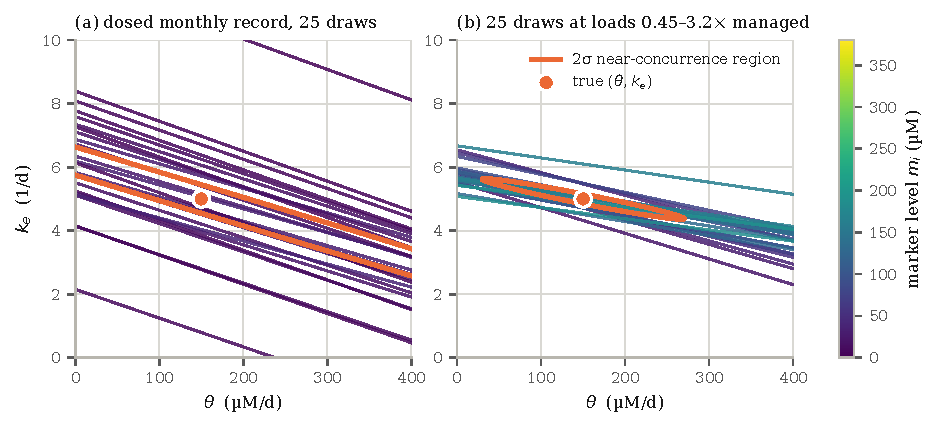
\includegraphics[width=\linewidth]{pi_pencil.pdf}
\caption{\label{sfig:pencil}Each settled blood draw as a line in the plane of residual
capacity $\theta$ (horizontal, \um) and the non-enzymatic rate constant $k_e$ (vertical,
d$^{-1}$), in the linear-clearance model for a patient at 5\% of normal (true
$\theta=150$\um, $k_e=5$\,d$^{-1}$, orange dot; normal capacity is 3000\um). Each coloured
line is one draw, $g(m_i)\theta+m_ik_e=L(t_i)+L_0-\Delta_ig(m_i)$; its slope is
$-1/(K_m+m_i)$ and its colour is the measured marker level $m_i$ (colour bar, \textmu M).
Without noise all lines would pass through the orange dot. The orange outline is the
$2\sigma$ region in which the lines nearly meet, drawn about the true point from the
noise-weighted normal matrix of the lines with $K_m=100$\uM\ and the unrecorded load known
and with no prior on $k_e$; assay coefficient of
variation 5\%, load-record error 5\%. (a)~The monthly design: 25 monthly draws over two
years on the assumed fortnightly dose train, with a 10\% day-to-day variation in the load;
marker 4.3--37.8\uM. All slopes are close to
$-1/K_m$, the lines run nearly parallel, and the $2\sigma$ region is a sliver that leaves
the plot on both sides; the two thick orange lines are its long edges, not draws. Along the
sliver a lower $\theta$ is offset by a higher $k_e$: the correlation of $\ln\theta$ with
$\ln k_e$ is $-0.998$ here, and $-0.99$ with $K_m$ and the load offset estimated and the
prior on $k_e$ applied, as in the main text.
$\operatorname{sd}(\ln\hat\theta)=2.73$. (b)~An imagined record, not a proposal: 25 untreated
draws, each at steady state under a daily load set between 0.45 and 3.2 times the usual one
(145--1033\um), marker 23.8--188.9\uM. The high-marker draws (blue-green) have flatter
slopes, the lines cross at an angle and the region closes into an ellipse;
$\operatorname{sd}(\ln\hat\theta)=0.40$. Loads at the upper end of this range lie far beyond
the carnitine model's tipping point, so the experiment is not admissible.}
\end{figure}
% src: audit/brief_2026-10-01/pi_note/pi_figs.py:67-91 (seeds 0 and 1, ellipse from the weighted normal matrix, no prior, fixed K_m); out/t51_pencil_geometry.txt:6-18 (:17 corr -0.998); out/t1_identifiability.txt:25 (corr -0.9919, K_m and b free, k_e prior); pi_note/figure_guide.tex:312-366

% -----------------------------------------------------------------------------
\subsection{The carnitine model}
\label{si:s1-carn}

\paragraph{The two-state system.} With $c(t)$ the carnitine available for conjugation
(\textmu M),
\begin{equation}
\label{seq:s1-twostate}
\begin{aligned}
\dot m &= L(t)+L_0-\bigl(\theta+\Delta(t)\bigr)g(m)-k\,c\,u(m),\\
\dot c &= R_0-k\,c\,u(m)-\delta(m)\,c,\qquad \delta(m)=\delta_0\Bigl(1+\frac{m}{M_i}\Bigr),
\end{aligned}
\end{equation}
with $u(m)=m/(K_c+m)$. $K_c$ is the half-saturation of the conjugation step, $k$ the
conjugation rate constant (d$^{-1}$), $R_0$ the constant replenishment of carnitine
(\um), $\delta_0$ the basal rate of carnitine loss other than by conjugation (d$^{-1}$), and
$M_i$ the metabolite level at which acylcarnitine competition doubles that loss. The
conjugation term enters both equations with the same coefficient, because one propionyl
group leaves with one carnitine. Carnitine also has an exit that the metabolite does not,
$\delta(m)c$, the filtered carnitine that is not recovered, and that exit widens as $m$
rises. Both features matter. If conjugation were carnitine's only exit, $\dot c=0$ would fix
the conjugation flux at $R_0$ for every $m$, so the flux would not vanish as the metabolite
does. With a second exit of constant rate the flux would vanish at $m=0$ and saturate at high
$m$; only a second exit that widens with $m$ makes it fall.
% src: manuscript/main.tex:612-621; paper/sections/03_dynamic.tex:36-70; src/common/models.py:193-216 (rhs_C), :145-164 (why the second exit)

\paragraph{The steady-state reduction.} Setting $\dot c=0$ gives
$c^{\ast}(m)=R_0/\bigl(k[u(m)+\rho(m)]\bigr)$ and the conjugation flux
\begin{equation}
\label{seq:s1-reduced}
\alpha_{\mathrm{carn}}(m)=k\,c^{\ast}(m)\,u(m)=\frac{R_0\,u(m)}{u(m)+\rho(m)},\qquad
\rho(m)=\rho_0\Bigl(1+\frac{m}{M_i}\Bigr),\quad \rho_0=\frac{\delta_0}{k},
\end{equation}
in which $k$ cancels. The flux vanishes at $m=0$, rises while the conjugation step fills,
and falls once competition outpaces it. The reduction is exact at every fixed point of the
two-state system, because $\dot c=0$ holds there, so steady states, the tipping point and
the critical capacity are computed exactly on equation~\eqref{seq:s1-reduced}. That the
two-state system, integrated from below the separatrix, settles on the reduced steady state
to fourteen digits is this identity and not an independent test.
% src: paper/sections/02_model.tex:113-146 (eq:alphaqss, exact by identity, fourteen digits); paper/sections/03_dynamic.tex:71-87

\paragraph{Away from steady state.} The reduction is not a fast--slow approximation.
Carnitine relaxes with time constant $\tau_c=1/\bigl(k[u(m)+\rho(m)]\bigr)$, 0.92\,d at
$k=1$\,d$^{-1}$ at the illustrative patient's steady state, against 0.81\,h for the marker
in the linear-clearance model at normal capacity, so carnitine is the slower state by a
factor of about 27; across the sampled region of the carnitine constants $\tau_c/\tau_m$
spans 0.52--55. Published human kinetics also put whole-body carnitine
turnover at 38--119\,h, with a rapidly equilibrating compartment of 2--3\,h~\cite{carnitine_turnover}.
The constant $k$ therefore cancels from the steady-state curve but sets how far the reduction
can be trusted away from it. Supplementary Table~\ref{stab:s1-kcost} gives the cost: the peak
relative error in $m$ of the reduced model against the two-state system after a step in the
load, with carnitine left at its value before the step. For this reason every dynamic
simulation (the late infusions of Supplementary Section~\ref{si:s7}) integrates the two-state
system, at $k=1$\,d$^{-1}$ (the model default) and at $k=10$\,d$^{-1}$ as a sensitivity case.
The basin of the stable state also differs between the two forms. Started with carnitine at
its value before a load rise (a fuller pool than $c^{\ast}$), the two-state system tolerates
excursions 10--18\% beyond the reduced separatrix across the sampled corners of the
constants; started with a depleted pool at 0.8, 0.5 and 0.25 times $c^{\ast}$, the boundary
falls 1.9\%, 4.8\% and 7.3\% below it at the nominal constants. The reduced separatrix is
therefore not a bound in either direction.
% src: paper/sections/02_model.tex:100-108 (0.92 d vs 0.81 h, factor 27, 38-119 h, 2-3 h), :134-137 (0.52 to 55), :156-170 (basin 10-18%, 1.9/4.8/7.3%); results/numbers/design.tex:110 (tau_hours 0.81); src/common/params.py:507-541 (k row)

\begin{table}[tbp]
\centering
\footnotesize
\caption{\label{stab:s1-kcost}Cost of the steady-state reduction away from steady state, as a
function of the conjugation rate constant $k$: peak relative error (\%) in the metabolite
level of the reduced model against the two-state system, after a step in the load to the
stated multiple of baseline, starting from the attractor at baseline load with carnitine
held at its value before the step. Carnitine model, nominal constants, illustrative patient
at 10\% of normal ($\theta=300$\um). At steady state the error is zero for every $k$.}
\begin{tabular}{@{}lcccc@{}}
\toprule
load step & $k=0.1$\,d$^{-1}$ & $k=1$\,d$^{-1}$ (default) & $k=10$\,d$^{-1}$ & $k=100$\,d$^{-1}$ \\
\midrule
illness, $1.50\times$ baseline & 83.1 & 31.8 & 4.8 & 0.5 \\
$1.10\times$ baseline & 18.4 & 9.9 & 1.9 & 0.2 \\
isotope-dilution tracer, $1.01\times$ baseline & 1.62 & 0.98 & 0.22 & 0.024 \\
\bottomrule
\end{tabular}
\end{table}
% src: results/numbers/reduction.tex:3-17 (generated by src/model_C/run.py, reduction_cost_numbers: ParamsC theta = 300, start at the baseline attractor, c at its pre-step value); src/common/params.py:515-535

\paragraph{How the replenishment rate is fixed.} $R_0$ is not a free constant. It is set so
that the non-enzymatic route alone peaks at 500\um\ against a baseline load of 600\um, so
that a patient with $\theta=0$ cannot be maintained, as the severity of null genotypes
requires. The peak has a closed form. Since $\alpha_{\mathrm{carn}}=R_0/(1+\rho/u)$ and
$\rho/u=\rho_0\bigl(K_c/m+1+K_c/M_i+m/M_i\bigr)$, the route peaks at
$m^{\ast}=\sqrt{K_cM_i}$, where
\begin{equation}
\label{seq:s1-R0}
\max_m\alpha_{\mathrm{carn}}=\frac{R_0}{1+\rho_0\bigl(1+\sqrt{K_c/M_i}\bigr)^{2}}
\quad\Longrightarrow\quad
R_0=500\,\bigl[1+\rho_0\bigl(1+\sqrt{K_c/M_i}\bigr)^{2}\bigr]\ \text{\um}.
\end{equation}
At the nominal $K_c=100$\uM, $M_i=300$\uM\ and $\rho_0=0.5$ this gives $R_0=1122.0$\um, with
the peak at $m^{\ast}=173$\uM. Because the peak depends on all three shape constants, $R_0$
is re-derived whenever $K_c$, $M_i$ or $\rho_0$ moves; holding $R_0$ fixed instead would
sweep parameter sets that break the model's own calibration and, at one end of each sweep,
make a patient with no enzyme maintainable.
% src: paper/sections/03_dynamic.tex:99-106 (calibration, re-derivation), :439-442; src/common/models.py:115 (R0 = 1122.0085); src/common/params.py:462-495 (R0 and ALT_peak rows). Closed form follows from eq. seq:reduced; it reproduces 1122.0085 at the nominal constants.

\paragraph{The tipping point and the intrinsic critical capacity.} Write
$C(m;\theta)=\theta g(m)+\alpha_{\mathrm{carn}}(m)$ for the total clearance at constant
capacity. Because $\alpha_{\mathrm{carn}}$ rises and then falls, $C$ has an interior
maximum, which increases with $\theta$. At a constant load $s$ above $\theta$, if
$\max_m C(m;\theta)>s$ the line $s$ cuts the curve twice: a stable steady state on the rising branch (the
attractor) and an unstable one on the falling branch (the separatrix). Above the separatrix
$\dot m>0$ even at the baseline load, so the metabolite keeps rising after the trigger has
gone; this is the tipping point. If $\max_m C<s$ there is no steady state and the
metabolite rises from any starting level. The intrinsic critical capacity is the capacity at
which the two steady states merge,
\begin{equation}
\label{seq:s1-thcint}
\thci(s)=\text{the unique }\theta\text{ with }\max_{m>0}C(m;\theta)=s ,
\end{equation}
unique because the maximum is continuous and strictly increasing in $\theta$. At the
baseline load of 600\um\ and the nominal constants, $\thci=150.8$\um, 5.0\% of normal. No
tolerable level enters this definition, unlike the threshold of the linear-clearance model
(equation~\eqref{seq:s1-thcritlin}). The threshold is positive only while the route alone
cannot carry the load, $\max_m\alpha_{\mathrm{carn}}<s$, which is what the calibration of
$R_0$ (500 against 600) secures. Under therapy the patient's capacity at the trough of the
dose cycle is $\theta+\dtr$, and the dosing interval is safe at baseline load while
$\theta+\dtr>\thci$ (Supplementary Section~\ref{si:s6:crossing}).
% src: paper/sections/03_dynamic.tex:369-437 (prop:intrinsic, argument, cor:fold); out/t53_crossing_shape.txt:5 (150.775); manuscript/main.tex:627-628,748-751. C(m) -> theta as m -> infinity (alpha_carn -> 0), so two crossings need s > theta.

For the illustrative patient at 10\% of normal ($\theta=300$\um), the attractor at baseline
load is at 82\uM\ and the separatrix at 1033\uM, and the largest load the patient can
balance at all is 706\um. A sustained rise of 18\% in the load is therefore the smallest
that strands this patient (Supplementary Fig.~\ref{sfig:s1-carnfold}). The separatrix sits
where $\alpha_{\mathrm{carn}}$ has decayed, on the scale of $M_i$, so the distance between
the two steady states depends on $M_i$ almost linearly (509 to 3275\uM\ over an eightfold
range of $M_i$), while its sign does not.
% src: out/t54_dose_timing.txt:73 (theta = 300 sits at 82 uM, separatrix 1033 uM); paper/sections/03_dynamic.tex:446-452 (706 vs 600; 18%), :484-492 (margin 509 to 3275 over eightfold M_i)

\begin{figure}[tbp]
\centering
\begin{minipage}[t]{0.49\linewidth}\centering
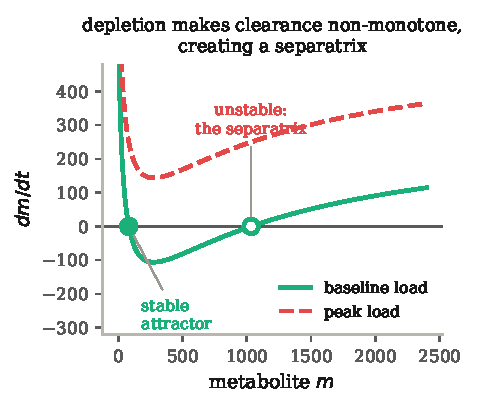
\includegraphics[width=\linewidth]{fig_C1_phaseline.pdf}
\end{minipage}\hfill
\begin{minipage}[t]{0.49\linewidth}\centering
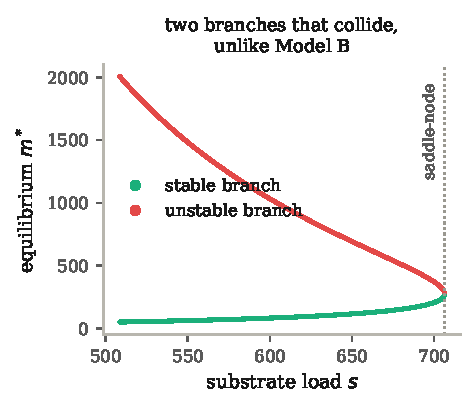
\includegraphics[width=\linewidth]{fig_C2_fold.pdf}
\end{minipage}
\caption{\label{sfig:s1-carnfold}The tipping point of the carnitine model, in its steady-state
form (equation~\eqref{seq:s1-reduced}), for the illustrative patient at 10\% of normal
($\theta=300$\um), nominal constants and no therapy. Metabolite $m$ in \textmu M; loads and
$dm/dt$ in \um. Left: the rate of change of the metabolite, $dm/dt=s-C(m)$, against $m$. At
the baseline load ($s=600$\um, solid) the curve crosses zero twice, at a stable attractor
(filled circle, 82\uM) and an unstable separatrix (open circle, 1033\uM); between them the
metabolite falls back to the attractor, beyond the separatrix it keeps rising. At a peak load
of 850\um\ (dashed) $dm/dt$ is positive at every level and there is no steady state.
Right: steady-state levels against a constant load. The stable branch (green) and the
unstable branch (red) approach and merge at the saddle-node (dotted line, 706\um), beyond
which no steady state exists. The in-figure title's ``Model~B'' is the saturable-clearance
model, in which the single steady state instead escapes to ever higher levels as the load
approaches the total maximal clearance $\theta+V_e$, without colliding with a second one.}
\end{figure}
% src: src/model_C/run.py:181-248 (fig_phaseline: s_base 600, s_peak 850, ParamsC theta = 300; fig_fold: loads 0.72-1.004 x fold); out/t54_dose_timing.txt:73; paper/sections/03_dynamic.tex:450

\paragraph{The unmeasured shape constants.} $K_c$, $M_i$ and $\rho_0$ have no measurement
behind them. We carry assumed ranges, $K_c$ 25--800\uM, $M_i$ 150--1200\uM\ and $\rho_0$
0.35--1, and re-derive $R_0$ at every point. One at a time, $\thci$ moves from 186.5 to
119.5\um\ as $K_c$ runs from 25 to 800\uM\ (a factor of 1.56), from 171.4 to 125.5\um\ as $M_i$
runs from 150 to 1200\uM\ (1.37), and from 149.7 to 152.1\um\ across the range of $\rho_0$.
At the eight corners of the three ranges it spans 109.9--232.1\um, a factor of 2.1; the
consequences for the dosing interval are in Supplementary Section~\ref{si:s6:corners}.
% src: out/t53_crossing_shape.txt:10,15,16,22,23,28 (one at a time), :76 (corners 109.9..232.1, factor 2.11); paper/sections/03_dynamic.tex:465-480

\paragraph{Validity limit.} The model predicts absolute urinary excretion of free carnitine
as the filtered load times the fraction not recovered, and the fraction not recovered rises
as $1+m/M_i$. Taking the filtered load as proportional to plasma free carnitine, which in a
child with PA was 5.7\uM\ against a normal $37\pm8$\uM~\cite{carnitine_pa_child}, the
filtered load is 6.5 times lower than normal and the predicted excretion falls, the direction
measured~\cite{carnitine_excretion_pa}. The prediction fails once $1+m/M_i$ exceeds
$37/5.7$, that is above $m\approx5.5\,M_i$: 1650\uM\ at the nominal $M_i$ and 825\uM\ at
$M_i=150$\uM. Simulated metabolite curves are stopped at this level.
% src: paper/sections/03_dynamic.tex:113-125 (excretion argument, 6.5, 5.5 M_i = 1650); REPORT.md:1169 (825 uM at the worst corner); manuscript/main.tex:628-629,776

% -----------------------------------------------------------------------------
\subsection{Parameter registry}
\label{si:s1-reg}

Supplementary Table~\ref{stab:params} lists every constant the main text and this
Supplementary Information use, with its value, its meaning, its status and what the value
rests on. Status is one of three classes: \emph{literature}, read from a cited source;
\emph{derived}, fixed by a constraint elsewhere in the model; and \emph{assumed}, chosen with
no measurement behind it, in which case the cost of the choice is reported where it matters.
Most constants are assumed, and the conclusions are stated relative to them; the rows on
which a conclusion turns are $\theta$ in the disease range, $k_e$ and its prior, $D$,
$t_{1/2}$ and the carnitine shape constants.
% src: src/common/params.py:13-41 (three source classes); :562-566

\begingroup
\footnotesize
\setlength{\LTcapwidth}{\linewidth}
\renewcommand{\arraystretch}{1.1}
\begin{longtable}{@{}>{\raggedright\arraybackslash}p{0.09\linewidth}
>{\raggedright\arraybackslash}p{0.15\linewidth}
>{\raggedright\arraybackslash}p{0.20\linewidth}
>{\raggedright\arraybackslash}p{0.10\linewidth}
>{\raggedright\arraybackslash}p{0.35\linewidth}@{}}
\caption{\label{stab:params}Parameter registry. Status: \emph{literature} (read from a cited
source), \emph{derived} (fixed by a constraint in the model) or \emph{assumed} (chosen, with
no measurement behind it). Ranges given for the carnitine shape constants are assumed ranges
of unmeasured constants, not published ranges.}\\
\toprule
symbol & value & meaning & status & what the value rests on \\
\midrule
\endfirsthead
\multicolumn{5}{@{}l}{\emph{Supplementary Table~\thetable, continued}}\\
\toprule
symbol & value & meaning & status & what the value rests on \\
\midrule
\endhead
\midrule
\multicolumn{5}{r@{}}{\emph{continued on the next page}}\\
\endfoot
\bottomrule
\endlastfoot
\multicolumn{5}{@{}l}{\emph{Shared by all three models}}\\
\addlinespace[2pt]
$\theta$ & 3000\um\ at normal & residual capacity: the maximal flux of the patient's own PCC & assumed (scale) &
sets the scale, chosen so that the carnitine model's illustrative 300\um\ is 10\% of normal;
the estimand, with no prior \\
$\theta_{\mathrm{PA}}$ & $\le150$\um\ ($\le5\%$) & capacity in severe PA & literature &
residual PCC activity in PA under 5\% of control~\cite{pcc_residual_activity}; fibroblast
enzymology, not hepatic capacity \\
$K_m$ & 100\uM & half-saturation of the enzyme term, at the plasma level & assumed &
not PCC's in vitro $K_m$ for propionyl-CoA, 0.29\,mM~\cite{pcc_liver_kinetics}; four PCC
variants share the wild-type $K_m$~\cite{pcc_variants_kinetics}, supporting one value
across capacities; no prior is used, and the record recovers it to 6--7\% at every capacity \\
$L_0$ (offset $b$) & unknown; prior sd 5\% of $L$ & unrecorded load & assumed (prior) &
prior mean zero, sd $0.05\times322.7=16.1$\um, a 95\% half-width of $\pm31.6$\um;
nothing measures it \\
$D$ & 6000\um & jump in delivered capacity at each fortnightly infusion (the assumed dose) &
assumed &
chosen so the marker falls by about two-thirds at peak effect (62--66\%, depending on the
baseline and peak used); the trial's reported falls after the third dose are smaller
($-29$, $-3$, $-20$, $+5$ and $-20\%$ across five cohorts, no dose
trend)~\cite{trial_phase12} \\
$D_{\mathrm{cap}}$ & 2672\um & largest jump within the ceiling at 14\,d and $t_{1/2}=3.5$\,d &
derived & $2850\,(1-e^{-14\lambda})$ \\
$t_{1/2}$ & 3.5\,d & half-life of the delivered PCC protein, in the identifiability and
sampling analyses & assumed &
a design value; the translational model's intrinsic PCC decay corresponds to 3.8\,d (row
below), and the only human measurement is 3.6\,d, in fibroblasts~\cite{chandler1985};
$\lambda=\ln2/t_{1/2}=0.198$\,d$^{-1}$ \\
& about 4.3\,d, plausibly 3--6\,d & likely hepatic half-life & literature (comparators) &
mouse liver mitochondrial proteins, median 4.26\,d~\cite{kim2012}; delivered human PCC in
mouse liver 5.3--6.7\,d~\cite{jiang2020dual}; translational model, intrinsic PCC decay
$k_{\deg}=0.0075$\,h$^{-1}$ (3.8\,d) inside a two-compartment protein model fitted in mice,
whose stated protein half-life is about 7\,d~\cite{pkpd_translational};
no human hepatic value is published \\
$T$ & 14\,d & interval between infusions & literature &
first dose group every three weeks, the four groups that followed every two
weeks~\cite{trial_phase12}; fortnightly schedule from model-informed dose
selection~\cite{gao2025acop} \\
$D\,\tau/14$ & & jump at interval $\tau$ & assumed (convention) &
same delivered amount per day at every interval (a 21-day infusion is 1.5 times a 14-day one) \\
ceiling & $\theta+\Delta\le3000$\um & own plus delivered capacity never above normal &
assumed (convention) & a plausibility condition, set for a patient at 5\% of normal
(delivered peak at most 2850\um); not a measured toxicity limit \\
\addlinespace
\midrule
\multicolumn{5}{@{}l}{\emph{Linear-clearance model}}\\
\addlinespace[2pt]
$k_e$ & 5\,d$^{-1}$ & rate constant of the non-enzymatic route & assumed &
no human measurement: the translational model has no marker state and no elimination
constant~\cite{pkpd_translational}, and the turnover structure publishes no
value~\cite{gao2025acop}; methylmalonic acid cleared by haemodialysis in one patient gives
4.41\,d$^{-1}$ at 70\,kg~\cite{ke_mma_analogue}, a dialytic figure that bounds the route from
above; the value used sits 13\% above it (the two coincide at 62\,kg); a marker half-life of
3.3\,h \\
$\bar m$ & 10\uM & marker level at normal capacity (operating point) & assumed &
design quantities are relative to it; the scale is murine (suppressible plasma 3-HP pool
60.1\uM\ in PCC-deficient mice~\cite{pkpd_translational}), within a factor of 1.6 of the
human newborn dried-blood-spot 99.9th centile, 38.13\,\textmu mol/L~\cite{dbs_3hp_cutoff} \\
$L$ & 322.7\um & recorded load at the operating point, held as capacity falls & derived &
$\theta g(\bar m)+k_e\bar m=272.7+50$ \\
load variation & 10\% (CV) & day-to-day variation of the recorded load & assumed &
ordinary variation in eating; it closes the load-bias identity (Section~\ref{si:s1-si}) \\
$m_{\mathrm{tol}}$ & 40\uM & tolerable metabolite level & assumed (convention) &
no numeric plasma 3-HP target is published; the only anchor is that a 50\% lower 3-HP
carries a decompensation rate ratio of 0.7~\cite{natural_history} \\
$f$ & 1.5, for 14\,d & illness amplitude as a multiple of baseline load & assumed &
muscle protein catabolism, indexed by 3-methylhistidine excretion, rises by 227--325\% in
sepsis and trauma in adults~\cite{muscle_catabolism}; muscle is only part of the propiogenic
load, so this is a loose bound \\
$\theta_{\mathrm{crit}}^{\mathrm{lin}}$ & 994\um\ ($f=1.5$); 430\um\ ($f=1$) & illness
threshold of this model & derived & equation~\eqref{seq:s1-thcritlin} \\
\addlinespace
\midrule
\multicolumn{5}{@{}l}{\emph{Carnitine model}}\\
\addlinespace[2pt]
$\theta$ (illustrative) & 300\um\ (10\%) & patient of Supplementary Fig.~\ref{sfig:s1-carnfold} &
assumed & chosen above $\thci$ \\
$s_{\mathrm{base}}$ & 600\um & baseline load & assumed (scale) &
not in physical units; the partition of propionate production is measured (amino acids
51.7\%, gut bacteria at least 22.2\%, about 30\% unaccounted)~\cite{propionate_sources} \\
$K_c$ & 100\uM\ (assumed range 25--800) & half-saturation of conjugation & assumed &
no measurement; the nearest analogue, the renal carnitine transporter ($K_m$ 0.08\,mM
external, 1.2\,mM internal), is a different step, measured in vitro in the
rat~\cite{octn2_renal_transport} \\
$M_i$ & 300\uM\ (assumed range 150--1200) & level at which acylcarnitine competition doubles
carnitine loss & assumed &
competition shown in vitro for the rat renal transporter~\cite{octn2_renal_transport}; no
propionylcarnitine inhibition constant is published \\
$\rho_0=\delta_0/k$ & 0.5 (assumed range 0.35--1) & basal carnitine loss relative to
conjugation & assumed &
below 1, since the carnitine drain in PA is dominated by
propionylcarnitine~\cite{carnitine_excretion_pa}; bounded below only by a direction \\
$\alpha_{\max}$ & 500\um & peak of the route alone & assumed (calibration) &
below $s_{\mathrm{base}}$ so that a patient with $\theta=0$ cannot be maintained (null
genotypes); ratio 0.833 \\
$R_0$ & 1122.0\um & carnitine replenishment & derived &
equation~\eqref{seq:s1-R0}; re-derived at every setting of $K_c$, $M_i$, $\rho_0$ \\
$k$ & 1\,d$^{-1}$ (10 as sensitivity) & conjugation rate constant & assumed &
cancels from the steady-state curve; nothing fixes it; it sets the carnitine time constant and
the off-equilibrium cost (Supplementary Table~\ref{stab:s1-kcost}) \\
$\delta_0$ & 0.5\,d$^{-1}$ & basal non-conjugative carnitine loss & derived & $\rho_0k$ \\
$\thci$ & 150.8\um\ (5.0\%); 109.9--232.1 over the corners & intrinsic critical capacity at
$s_{\mathrm{base}}$ & derived & equation~\eqref{seq:s1-thcint} \\
validity limit & $5.5\,M_i=1650$\uM & highest level at which the model's carnitine
excretion is consistent with measurement & derived &
plasma free carnitine 5.7 against $37\pm8$\uM~\cite{carnitine_pa_child} \\
\addlinespace
\midrule
\multicolumn{5}{@{}l}{\emph{Saturable-clearance model}}\\
\addlinespace[2pt]
$V_e$ & 400\um\ nominal; 100\um\ at the constructed point & maximal rate of the
non-enzymatic route & assumed &
no source and no row in the model's own registry; at 400\um\ the route alone exceeds the
anchored load (285.6\um), so $\theta=0$ is maintainable; 100\um\ is chosen below the
untreated load (about 276\um) \\
$K_e$ & 300\uM & half-saturation of the route & assumed &
no source; a lumped route of several processes may have no single half-saturation; in this
model the target is touched only with $V_e$ from the intravenous tracer and $K_e$ known to
about 30\% (Supplementary Section~\ref{si:s4:sat}) \\
managed load & 220\um & load at the constructed point & assumed &
about 20\% below the untreated load; admits a steady state at 5\% of normal with a margin of
about 1\% of normal \\
\addlinespace
\midrule
\multicolumn{5}{@{}l}{\emph{Measurement, priors and target}}\\
\addlinespace[2pt]
CV & 5\% & analytical coefficient of variation of the marker assay & assumed &
no analytical figure for plasma 3-HP in PA was found; the nearest published repeatability,
a between-visit breath-test CV of $14.02\pm12.86\%$ in methylmalonic
acidaemia~\cite{breath_test_mma}, is for a different measurement \\
$\sigma_L/L$ & 5\% & relative error of the recorded load at each visit & assumed &
measurable by a weighed intake study; none exists in PA, where records are usually
prescriptions rather than intake as eaten \\
$s_{\ln k_e}$ & 0.8 (a factor of 2.23) & sd of the log-normal prior on $k_e$ & assumed (prior) &
no source; the target still holds up to a factor of 2.67; without the prior, the densest
design (draws every two days for two years, normal capacity) gives 1.11 instead of 0.150 \\
target & $\sdl{\hat\theta}=0.20$ & precision taken as useful (about $\pm20\%$) & assumed
(convention) & a design target, not a clinical requirement \\
settling window & first hour after an infusion & draws excluded from the steady-state fit &
assumed & the marker relaxes with a time constant of about 0.8\,h at normal capacity \\
\end{longtable}
\endgroup
% src: src/common/params.py:101-111 (M_OP, M_TOL, ILLNESS_FOLD, ASSAY_CV, S_BASE_C, ALT_PEAK_C, KE_PRIOR_LOG, LOAD_FRAC), :134-153 (theta), :154-175 (theta_PA), :176-200 (K_m, 0.29 mM), :201-251 (k_e, 4.41/d at 70 kg, 3.3 h; results/numbers ke_mma_vs_carried_pct 13, ke_mma_cross_bw 62), :252-259 (m_tol), :260-273 (illness fold, 227-325%), :283-300 (lambda), :301-306 (T_dose), :307-325 (D: 62-66%, trial falls), :351-369 (CV, 14.02 +/- 12.86%), :370-390 (s_ln_ke 0.8, factor 2.23), :391-401 (sigma_L/L), :420-428 (K_m shared, variants), :429-438 (K_c, 0.08 and 1.2 mM), :439-451 (M_i), :452-461 (rho_0), :462-495 (R0, ALT_peak, ratio 0.833), :496-506 (s_base), :507-542 (k)
% src: src/common/models.py:68-83,87-115 (ParamsA, ParamsB, ParamsC values); results/numbers/design.tex:42 (ke_needed_factor 2.67), :64-65 (sd_dense 0.1500, sd_dense_flat 1.1096), :110 (tau_hours 0.81); out/t18_set_id.txt:23 (sd ln K_m 0.062); out/t53_crossing_shape.txt:5,76 (theta_crit_int; corners), :65 (D = 2672); out/t44_interval_decision.txt:40,64 (994, 430); manuscript/main.tex:405-407 (3.6 d, 4.26 d, 4.3 d, 3-6 d), :654 (3.5 d assumed; 3.8 d intrinsic), :755 (2850), :350-352 (V_e from the tracer, K_e to about 30%); audit/brief_2026-10-01/REPORT.md:1004, 1021-1024 (Chandler 3.6 d; Jiang 5.3-6.7 d; Attarwala 0.0075/h in mouse, 3.8 d intrinsic, ~7 d effective terminal), :752-774 (V_e, K_e unregistered; 285.6; 276; managed 220), :798 (K_e to ~30%); trial_phase12 dosing (manuscript/main.tex:100-101)
